\documentclass{article}

% Symbols
%\usepackage{recycle}
\usepackage{amsfonts, amsthm}
\usepackage{upgreek}
\usepackage{physics}
\usepackage{cancel}
\usepackage{amssymb, latexsym, amsmath}

% Proof
\renewcommand*{\proofname}{\textbf{Demostraci\'on:}}

% Graphics
\usepackage{graphicx}
\usepackage{pgf}

% Color a letras.
%\usepackage[usenames,dvipsnames,svgnames,table]{xcolor}

% Tikz
\usepackage{tikz}
\usetikzlibrary{arrows,automata}
\usepackage{tikz}
\usetikzlibrary{arrows,automata}

\usetikzlibrary{shapes,calc}
\tikzstyle{edge}=[shorten <=2pt, shorten >=2pt,
  >=stealth, line width=1.1pt]
\tikzstyle{blueE}=[shorten <=2pt, shorten >=2pt,
  >=stealth, line width=1.5pt, blue]
\tikzstyle{blackV}=[circle, fill=black,
  minimum size=6pt,
  inner sep=0pt, outer sep=0pt]
\tikzstyle{blueV}=[circle, fill=blue, draw,
  minimum size=6pt, line width=0.75pt,
  inner sep=0pt, outer sep=0pt]
\tikzstyle{redV}=[circle, fill=red, draw,
  minimum size=6pt, line width=0.75pt,
  inner sep=0pt, outer sep=0pt]
\tikzstyle{redSV}=[semicircle, fill=red, minimum
  size=3pt, inner sep=0pt, outer sep=0pt,
  rotate=225]
\tikzstyle{blueSV}=[semicircle, fill=blue, minimum
  size=3pt, inner sep=0pt, outer sep=0pt,
  rotate=225]
\tikzstyle{blackSV}=[semicircle, fill=black, minimum
  size=3pt, inner sep=0pt, outer sep=0pt,
  rotate=225]
\tikzstyle{vertex}=[circle, draw, minimum size=6pt,
  line width=0.75pt, inner sep=0pt,
  outer sep=0pt]

% Margins
%Margins
\addtolength{\voffset}{-1cm}
\addtolength{\hoffset}{-1cm}
\addtolength{\textwidth}{2cm}
\addtolength{\textheight}{2cm}
%Header-Footer
\usepackage{fancyhdr}
\renewcommand{\headrulewidth}{1pt}

\newcommand{\set}[1]{%
  \left\{ #1 \right\}%
}

%\pagenumbering{gobble} -- Este comando
%                       -- quita el número de página.
\footskip = 50pt
\renewcommand{\headrulewidth}{1pt}

\pagestyle{fancyplain}

\begin{document}
  \title{UNIVERSIDAD AUT\'ONOMA DE M\'EXICO\\ Facultad de Ciencias}
  \author{Autores:
    \\ Fernanda Villaf\'an Flores
    \\ Fernando Alvarado Palacios
    \\ Adri\'an Aguilera Moreno}
  \date{}
  \maketitle
  \begin{center}
    
\includegraphics[scale=0.20]{../Imagen/Portada.jpg}\\[0.4cm]
    \Large
    \bf{Gr\'aficas y Juegos}
    \normalsize
  \end{center}
  \newpage
  \fancyhead[r]{ Gr\'aficas y Juegos 2022-1}
  \section*{\LARGE{Tarea 3}}

  \begin{enumerate}
    %%%%%%%%%%%%%%%%%%%%%%%%%%%%%%%%%%% Ejercicio 01 %%%%%%%%%%%%%%%%%%%%%%%%%%%%%%%%%%%
    \item Demuestre que si $e \in E$, entonces $c(G) \le c(G-e) \le c(G) + 1$.

      \renewcommand\qedsymbol{QED}
      \begin{proof}
        Dado que $c$ corresponde a la función que devuelve la cantidad de componentes
        conexas, analicemos dos casos posibles:

        \begin{itemize}
        \item[-] Si ``e" no es un puente, entonces:
          \begin{equation}
            c(G -e) = c(G)
          \end{equation}
          Esto pues sabemos que al borrarla una arista  que no es puente, $G$ no cambia en
          número de componentes conexas y así:
          \begin{equation}
            c(G) \leq c(G -e)
          \end{equation}
          De la dicotomia de $\leq$, sabemos que cumple con la igualdad. \\
          Luego, hacemos notar que:
          \begin{eqnarray}
            c(G) < c(G) +1\\
            \Rightarrow c(G) \leq c(G) +1
          \end{eqnarray}
          De $1$ y $4$ se sigue que:
          \begin{equation}
            c(G -e) \leq c(G) +1
          \end{equation}
          De $2$ y $5$ tenemos que:
          \[
          c(G) \le c(G-e) \le c(G) + 1
          \]

        \item[-] Si ``e" es un puente, entonces:
          \begin{equation}
            c(G) < c(G -e) \text{, por la definición de arista como puente}
          \end{equation}

          Así, tenemos que:
          \begin{equation}
            c(G) \leq c(G -e) \text{, pues de la dicotomia se cumple con $<$}
          \end{equation}

          Además, sabemos que el número de componentes conexas aumenta exactamente en
          $1$ en $G -e$ (porque estamos trabajando con gráficas simples). \\
          De esto, se sigue que:
          \begin{eqnarray}
            c(G -e) = c(G) +1\\
            \Rightarrow c(G -e) \leq c(G) +1
          \end{eqnarray}
          De $7$ y $9$ se sigue que:
          \[
          c(G) \le c(G-e) \le c(G) + 1
          \]
        \end{itemize}
        De lo anterior, concluimos que $c(G) \le c(G-e) \le c(G) + 1$. \\
      \end{proof}

  %%%%%%%%%%%%%%%%%%%%%%%%%%%%%%%%%%% Ejercicio 02 %%%%%%%%%%%%%%%%%%%%%%%%%%%%%%%%%%%
  \item Una gr\'afica es \textit{escindible completa} si su conjunto de
    v\'ertices admite una partici\'on $(S,K)$ de tal forma que $S$ es un
    conjunto independiente, $K$ es un clan, y cada v\'ertice en $S$ es adyacente
    a cada v\'ertice en $K$. Demuestre que una gr\'afica es escindible
    completa si y s\'olo si no contiene a $C_4$ ni a $\overline{P_3}$ como
    subgr\'afica inducida. 
    
    \renewcommand\qedsymbol{QED}
    \begin{proof}
      Sea $C_4 = (x_0, x_1, x_2, x_3, x_0)$ y $\overline{P_3} = \{y_0, y_1, y_2\}$
      tal que $y_0 y_2 \in E_G$, $y_0 y_1, y_1 y_2 \notin E_G$ \footnote{Sin pérdida de generalidad.}
      , con $x_i, y_j \in V_G$ ($0 \leq i \leq 3$, $0 \leq j \leq 2$). 
      N\'otese que los $x_i$'s, $y_j$'s no pueden estar contenidos en una misma parte. 
      Es decir, $C_4$ y $\overline{P_3}$ no est\'an contenidos en $S$ (ya que ning\'un
      v\'ertice en $S$ es adyacente). De igual manera, no est\'an contenidos en $K$
      (ya que para cualesquiera $3$ o $4$ v\'ertices en $K$ se tiene a $K_3$ o $K_4$).

      Para este ejercicio analizaremos dos posibles casos:
      \begin{itemize}
        \item[$\Rightarrow$)] Procedamos por reducción al absurdo.
          \begin{itemize}
            \item[$\cdot$)] Si $G$ es \textit{escendible completa}, entonces $C_4$ es
              subgr\'afica inducida de $G$.
              Supongamos, sin p\'erdida de generalidad, que $x_0 \in S$ y $x_1 \in K$
              (caso contrario, $x_1 \in S$ y $x_0$ no ser\'ia adyacente a $x_1$!!).
              Luego, si $x_2 \in S$ entonces $x_3 \in K$ (caso contrario, $x_3 \in S$
              y $x_2$ no ser\'ia adyacente a $x_3$!!). 
              As\'i por definici\'on de $K$ (clan), $x_1 x_3 \in E_G$!!
              (ya que $x_1, x_3 \in K$). 
              Si $x_2 \in K$, entonces $x_3 \in S$ (caso contrario, $x_3 \in K$ y
              $x_1 x_3 \in E_G$!!). Pero $x_0$ no es adyacente a $x_3$!! ($x_0, x_3
              \in S$). He aqu\'i una contradicci\'on de suponer a $C_4$ como subgr\'afica
              inducida de $G$.
              Por tanto, se concluye que $C_4$ no est\'a contenida como subgr\'afica
              inducida en $G$. 

            \item[$\cdot\cdot$)] Si $G$ es \textit{escendible completa}, entonces
              $\overline{P_3}$ es subgr\'afica inducida de $G$. 
              Supongamos, sin pérdida de generalidad, que $y_0 \in S$. 
              Entonces: $y_1 \in S$ (pues $y_0 y_1 \notin E_G$).
              Luego, $y_2 \in S$!! (pues $y_1 y_2 \notin E_G$). Pero no todos los $y_i$'s
              pueden estar en $S$. 
              Si $y_0 \in K$, entonces $y_1 \in S$ o $y_1 \in K$ implican que $y_0$ es
              adyacente a $y_1$!! 
              Pero $y_0 y_1 \notin E_G$ y he aqu\'i una contradicci\'on de suponer a
              $\overline{P_3}$
              como subgr\'afica inducida de $G$.
              Por tanto, se concluye que $\overline{P_3}$ no est\'a contenida como
              subgr\'afica inducida en $G$.
          \end{itemize}

        \item[$\Leftarrow$)] Para este caso, analicemos a todas las gr\'aficas no isomorfas
          que no son $\overline{P_3}$ con $3$ v\'ertices y no son $C_4$ con $4$ v\'ertices.

          \textbf{Con 3 v\'ertices:}

          \begin{figure}[ht!]
            \centering
            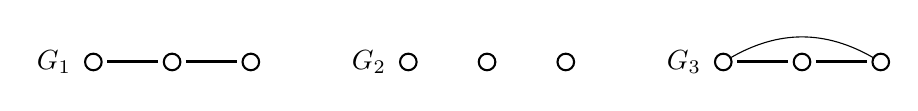
\begin{tikzpicture}
              %%%%%  Componente izquierda  %%%%%
              \node (0) [vertex,label=180:] at (0,1){};
              \node (1) [vertex,label=90:]  at (1,1){};
              \node (2) [vertex,label=90:]  at (2,1){};

              \draw [edge] (0) to (1);
              \draw [edge] (1) to (2);

              \node (L) at (-0.5,1){$G_1$};

              %%%%% Componente centro  %%%%%%%
              \begin{scope}[xshift=4cm]
                \node (9) [vertex,label=180:]  at (0,1){};
                \node (10) [vertex,label=90:]  at (1,1){};
                \node (11) [vertex,label=90:]  at (2,1){};

                \node (L) at (-0.5,1){$G_2$};
              \end{scope}

              %%%%% Componente derecha  %%%%%%
              \begin{scope}[xshift=8cm]
                \node (0) [vertex,label=180:] at (0,1){};
                \node (1) [vertex,label=90:]  at (1,1){};
                \node (2) [vertex,label=90:]  at (2,1){};

                \draw [edge] (0) to (1);
                \draw [edge] (1) to (2);
                \path(0)edge[bend left]node{}(2);

                \node (L) at (-0.5,1){$G_3$};
              \end{scope}
            \end{tikzpicture}
          \end{figure}


          \textbf{Con 4 vértices:}

          \begin{figure}[ht!]
            \centering
            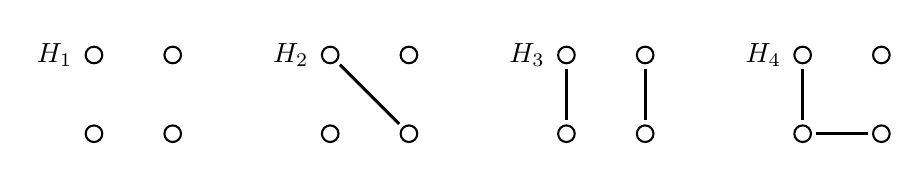
\begin{tikzpicture}
              %%%%%  Componente izquierda  %%%%%
              \node (0) [vertex,label=180:] at (0,1){};
              \node (1) [vertex,label=90:]  at (1,1){};
              \node (2) [vertex,label=90:]  at (0,0){};
              \node (3) [vertex,label=90:]  at (1,0){};

              \node (L) at (-0.5,1){$H_1$};

              %%%%% Componente centro 1  %%%%%%%
              \begin{scope}[xshift=3cm]
                \node (4) [vertex,label=180:] at (0,1){};
                \node (5) [vertex,label=90:]  at (1,1){};
                \node (6) [vertex,label=90:]  at (0,0){};
                \node (7) [vertex,label=90:]  at (1,0){};

                \draw [edge] (4) to (7);
                \node (L) at (-0.5,1){$H_2$};
              \end{scope}

              %%%%% Componente centro 2  %%%%%%
              \begin{scope}[xshift=6cm]
                \node (8)  [vertex,label=180:] at (0,1){};
                \node (9)  [vertex,label=90:]  at (1,1){};
                \node (10) [vertex,label=90:]  at (0,0){};
                \node (11) [vertex,label=90:]  at (1,0){};

                \draw [edge] (8) to (10);
                \draw [edge] (9) to (11);
                \node (L) at (-0.5,1){$H_3$};
              \end{scope}

              %%%%% Componente derecha  %%%%%%
              \begin{scope}[xshift=9cm]
                \node (12)  [vertex,label=180:] at (0,1){};
                \node (13)  [vertex,label=90:]  at (1,1){};
                \node (14) [vertex,label=90:]   at (0,0){};
                \node (15) [vertex,label=90:]   at (1,0){};

                \draw [edge] (12) to (14);
                \draw [edge] (14) to (15);
                \node (L) at (-0.5,1){$H_4$};
              \end{scope}
            \end{tikzpicture}
          \end{figure}

          \begin{figure}[ht!]
            \centering
            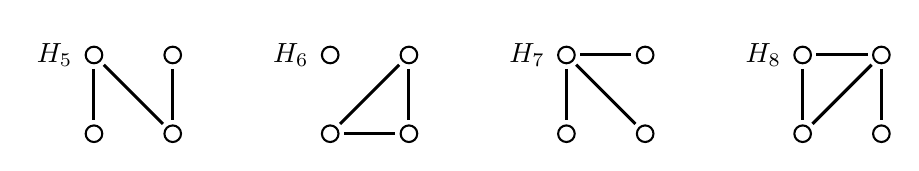
\begin{tikzpicture}
              %%%%%  Componente izquierda  %%%%%
              \node (0) [vertex,label=180:] at (0,1){};
              \node (1) [vertex,label=90:]  at (1,1){};
              \node (2) [vertex,label=90:]  at (0,0){};
              \node (3) [vertex,label=90:]  at (1,0){};

              \draw [edge] (0) to (2);
              \draw [edge] (0) to (3);
              \draw [edge] (1) to (3);
              \node (L) at (-0.5,1){$H_5$};

              %%%%% Componente centro 1 %%%%%%%
              \begin{scope}[xshift=3cm]
                \node (4) [vertex,label=180:] at (0,1){};
                \node (5) [vertex,label=90:]  at (1,1){};
                \node (6) [vertex,label=90:]  at (0,0){};
                \node (7) [vertex,label=90:]  at (1,0){};

                \draw [edge] (5) to (6);
                \draw [edge] (5) to (7);
                \draw [edge] (6) to (7);
                \node (L) at (-0.5,1){$H_6$};
              \end{scope}

              %%%%% Componente centro 2  %%%%%%
              \begin{scope}[xshift=6cm]
                \node (8)  [vertex,label=180:] at (0,1){};
                \node (9)  [vertex,label=90:]  at (1,1){};
                \node (10) [vertex,label=90:]  at (0,0){};
                \node (11) [vertex,label=90:]  at (1,0){};

                \draw [edge] (8) to (9);
                \draw [edge] (8) to (10);
                \draw [edge] (8) to (11);
                \node (L) at (-0.5,1){$H_7$};
              \end{scope}

              %%%%% Componente derecha  %%%%%%
              \begin{scope}[xshift=9cm]
                \node (12) [vertex,label=180:]  at (0,1){};
                \node (13) [vertex,label=90:]   at (1,1){};
                \node (14) [vertex,label=90:]   at (0,0){};
                \node (15) [vertex,label=90:]   at (1,0){};

                \draw [edge] (12) to (13);
                \draw [edge] (12) to (14);
                \draw [edge] (13) to (14);
                \draw [edge] (13) to (15);
                \node (L) at (-0.5,1){$H_8$};
              \end{scope}
            \end{tikzpicture}
          \end{figure}

          \begin{figure}[ht!]
            \centering
            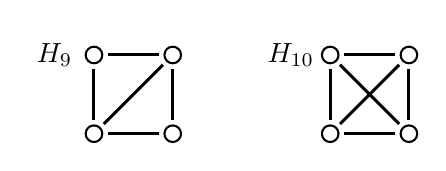
\begin{tikzpicture}
              %%%%%  Componente izquierda  %%%%%
              \node (0) [vertex,label=180:] at (0,1){};
              \node (1) [vertex,label=90:]  at (1,1){};
              \node (2) [vertex,label=90:]  at (0,0){};
              \node (3) [vertex,label=90:]  at (1,0){};

              \draw [edge] (0) to (1);
              \draw [edge] (0) to (2);
              \draw [edge] (1) to (2);
              \draw [edge] (1) to (3);
              \draw [edge] (2) to (3);
              \node (L) at (-0.5,1){$H_9$};

              %%%%% Componente derecha %%%%%%%
              \begin{scope}[xshift=3cm]
                \node (4) [vertex,label=180:] at (0,1){};
                \node (5) [vertex,label=90:]  at (1,1){};
                \node (6) [vertex,label=90:]  at (0,0){};
                \node (7) [vertex,label=90:]  at (1,0){};

                \draw [edge] (4) to (5);
                \draw [edge] (4) to (6);
                \draw [edge] (4) to (7);
                \draw [edge] (5) to (6);
                \draw [edge] (5) to (7);
                \draw [edge] (6) to (7);
                \node (L) at (-0.5,1){$H_{10}$};
              \end{scope}
            \end{tikzpicture}
          \end{figure}
          
          
          Propongamos la partición $(S, K)$ en $G$.

          Notemos que $H_2, H_3, H_4, H_5, H_6$, y $H_8$ contienen como subgr\'aficas inducidas a
          $\overline{P_3}$. \\
          Luego, s\'olo $H_1, H_7, H_9$, y $H_{10}$ junto a $G_1, G_2$, y $G_3$
          son subgr\'aficas inducidas de $G$ y podemos hacer el siguiente an\'alisis:

          \begin{itemize}
            \item[$1$)] $G_2$ y $H_1$ est\'an contenidas como subgráficas inducidas en $S$.

            \item[$2$)] $G_1$ tiene los $2$ v\'ertices de grado $1$ en $S$ y el \'unico
              v\'ertice de grado $2$ est\'a en $K$.

            \item[$3$)] $G_3$ y $H_{10}$ est\'an en $K$.

            \item[$4$)] $H_7$ tiene a su \'unico v\'ertice de grado $3$ en $K$ y el resto de
              sus v\'ertices est\'a en $S$.

            \item[$5$)] $H_9$ tiene a sus $2$ v\'ertices de grado $2$ en $S$ y al resto en $K$.
          \end{itemize}

          Con base a lo anterior, podemos sugerir que $K$ es un clan y $S$ es independiente y
          ambos subconjuntos de $V_G$. Con esto tenemos que $G$ es \textit{escindible}.
          
          Por ($2$), ($4$) y ($5$), vemos que es necesario que haya aristas entre v\'ertices de $S$
          y $K$. Como ($1$) y ($3$) no restringen la condición anterior, entonces se puede
          considerar a \textit{escindible completa}.
      \end{itemize}

      De los casos anteriores, concluimos que una gr\'afica es escindible completa si y s\'olo si
      no contiene a $C_4$ ni a $\overline{P_3}$ como subgr\'afica inducida.
    \end{proof}

  %%%%%%%%%%%%%%%%%%%%%%%%%%%%%%%%%%% Ejercicio 03 %%%%%%%%%%%%%%%%%%%%%%%%%%%%%%%%%%%
  \item \begin{enumerate}

    %%%%%%%%%%%%%%%%%%%%% ---------- 03 (a)
    \item Demuestre que si $|E| > {|V|-1 \choose 2}$, entonces $G$ es conexa.

      \renewcommand\qedsymbol{QED}
      \begin{proof}
        Si $|E_G| = {|V| -1 \choose 2}$, entonces hay dos posibilidades:

        \begin{itemize}
          \item[-] Si $G$ es conexa, entonces $G+e$ (con $e \in E_G$) cumple que:
            \begin{eqnarray*}
              |E_{G +e}| &=& {|V| -1 \choose 2} +1\\
              &>& {|V| -1 \choose 2}
            \end{eqnarray*}
            Además, $e$ no es ni lazo ni arista multiple,
            pues sabemos de resultados vistos en clase que una gráfica es completa si
            $|E| = {|V| \choose 2}$ y como
            \begin{eqnarray*}
              {|V| \choose 2} \not= {|V| -1 \choose 2}
            \end{eqnarray*}
            ya que
            \begin{eqnarray*}
              {|V| \choose 2} = \frac{n \cdot (n -1)}{2}
            \end{eqnarray*}
            y
            \begin{eqnarray*}
              {|V| -1 \choose 2} = \frac{(n -1) \cdot (n -2)}{2}
            \end{eqnarray*}
            Luego,
            \begin{eqnarray*}
              {|V| \choose 2} &\not=& {|V| -1 \choose 2}\\
              \frac{n \cdot (n -1)}{2} &\not=& \frac{(n -1) \cdot (n -2)}{2}\\
              n \cdot (n -1) &\not=& (n -1) \cdot (n -2)\\
              n &\not=& n -2
            \end{eqnarray*}
            y de hecho
            \begin{eqnarray*}
              {|V| \choose 2} > {|V| -1 \choose 2}
            \end{eqnarray*}
            Así, se justifica que $e$ no sea ni lazo ni arista multiple.
            
            De lo anterior, se sigue que $G +e$ es una gráfica simple que además es conexa,
            pues $G$ ya es conexa.

          \item[-] Si $G$ no es conexa, entonces existe un vértice aislado $x$, ya que:
            \begin{eqnarray*}
              {|V| -1 \choose 2} &=& \frac{|V_G|^2 -|V_G| -2 \cdot |V| +2}{2}\\
              &=& \frac{|V_G|^2 -|V_G|}{2} + \frac{2 -2|V_G|}{2}\\
              &=& \frac{|V_G| \cdot (|V_G| -1)}{2} - \frac{\cancel{2} \cdot (|V_G| -1)}{\cancel{2}}\\
              &=& {|V_G| \choose 2} - (|V_G| -1)
            \end{eqnarray*}
            Sabemos por resultados vistos en clases que hay ${|V_G| \choose 2}$ aristas en
            una gráfica completa y un vértice puede relacionarse a lo más con $|V_G| -1$ vértices
            (pues estamos trabajando con gráficas simples).
            
            Nótese que de lo anterior se infiere que $G - \{x\}$ es conexa
            \footnote{Esto ya que $|E_{G - \{x\}}| = {|V_G| \choose 2}$.}
            y así $G + e$ (con $e \in E_G$)
            \begin{eqnarray*}
              |E_{G +e}| &=& {|V| -1 \choose 2} +1\\
              &>& {|V| -1 \choose 2}
            \end{eqnarray*}
            es conexa, pues no hay lazos y no hay aristas múltiples en $G$.

            Entonces, tenemos que la nueva arista está comprendida entre $x$ y algún otro
            vértice en $V_{G - \{x\}}$. Por lo que habrá una $xy$-trayectoria para $y \in E_G$.
        \end{itemize}
        De lo anterior, concluimos que
        $|E_G| > {|V| -1 \choose 2} \Rightarrow G \text{ es conexa.}$ 
      \end{proof}

    %%%%%%%%%%%%%%%%%%%%% ---------- 03 (b)
    \item Para $|V| > 1$ encuentre una gr\'afica inconexa con $|E| = {|V|-1
      \choose 2}$.

      \textbf{\textit{Solución:}}

      Si $|V_G| = 2$, como $2 > 1 \Rightarrow |V_G| > 1$. \\
      Luego la gráfica que tiene como vértices a $u$ y $v$ y además:
      \begin{eqnarray*}
        |E_G| &=& {2 -1 \choose 2}\\
        &=& \frac{(2 -1) \cdot (2 -2)}{2}\\
        &=& 0
      \end{eqnarray*}

      A continuación se muestra la gráfica mencionada:

      \begin{figure}[ht!]
        \centering
        \begin{tikzpicture}
          \node (0) [vertex,label=90:$u$] at (1,0){};
          \node (1) [vertex,label=90:$v$]  at (6,0){};
          \node (L) at (-0.5,1){$G_1$};
        \end{tikzpicture}
      \end{figure}

      Así, observemos que la gráfica anterior es inconexa.

      \hfill $\square$
  \end{enumerate}

  %%%%%%%%%%%%%%%%%%%%%%%%%%%%%%%%%%% Ejercicio 04 %%%%%%%%%%%%%%%%%%%%%%%%%%%%%%%%%%%
  \item \begin{enumerate}

    %%%%%%%%%%%%%%%%%%%% ----------- 04 (a)
    \item Demuestre que si $\delta > \lfloor \frac{|V|}{2} \rfloor - 1$,
      entonces $G$ es conexa.

      \renewcommand\qedsymbol{QED}
      \begin{proof}
        Para este inciso procedemos por inducción sobre $V_G$. \\
        Sea $G$ una gráfica con $|V_G| = 1$. \\
        Así, $\delta = \lfloor \frac{1}{2} \rfloor = 0$, \textit{i.e.},

        \begin{figure}[ht!]
          \centering
          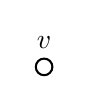
\begin{tikzpicture}
            \node (0) [vertex,label=90:$v$]  at (0,0){};
          \end{tikzpicture}
        \end{figure}

        donde $E_G = \varnothing$.
        
        Luego, supongamos como hipótesis inductiva que para una cantidad $n$ de
        vértices, el que se cumpla $\delta = \lfloor \frac{|V|}{2} \rfloor$ implica
        que $G$ es conexa.
        
        A continuación veamos qué pasa con $G + \{x\}$, donde $x \in V_{G + \{x\}}$.
        Así, $G$ cumple con $\delta = \lfloor \frac{|V|}{2} \rfloor$.
        
        De lo anterior, se sigue que $x$ es vecino de al menos $\lfloor \frac{|V|}{2}
        \rfloor$ vértices en $G$ (notemos que $G$ es, de hecho, una subgráfica inducida
        por vértices de $G +\{x\}$). Como $G$ es conexa, por hipótesis inductiva se sigue
        que $G + \{x\}$ es conexa. 
      \end{proof}

    %%%%%%%%%%%%%%%%%%%% ----------- 04 (b)
    \item Para $|V|$ par encuentre una gr\'afica $(\lfloor \frac{|V|}{2}
      \rfloor -1)$-regular e inconexa.

      \textbf{\textit{Solución:}}

      Con $|V| = 4$, tenemos que:
      \begin{eqnarray*}
        \lfloor \frac{4}{2} \rfloor -1 &=& 2 -1\\
        &=& 1
      \end{eqnarray*}

      \begin{figure}[ht!]
        \centering
        \begin{tikzpicture}
          \node (0) [vertex,label=90:$a$]  at (1,0){};
          \node (1) [vertex,label=90:$b$]  at (6,0){};
          \node (2) [vertex,label=90:$a$]  at (1,-2){};
          \node (3) [vertex,label=90:$b$]  at (6,-2){};

          \node (L) at (-0.5,1){$G$};

          \draw [edge] (0) to (1);
          \draw [edge] (2) to (3);
        \end{tikzpicture}
      \end{figure}

      Así, la gráfica es $1$-regular e inconexa.

      \hfill $\square$
  \end{enumerate}

  %%%%%%%%%%%%%%%%%%%%%%%%%%%%%%%%%%% Ejercicio 05 %%%%%%%%%%%%%%%%%%%%%%%%%%%%%%%%%%%
  \item Demuestre que si $D$ no tiene lazos y $\delta^+ \ge 1$, entonces $D$
    contiene un ciclo dirigido de longitud al menos $\delta^+ + 1$.

    \renewcommand\qedsymbol{QED}
    \begin{proof}
      Para este ejercicio procedamos por inducción en $V$.
      Así, cuando $\delta^+ = 1$ y $|V| = 2$ tendremos que:

      \begin{center}
        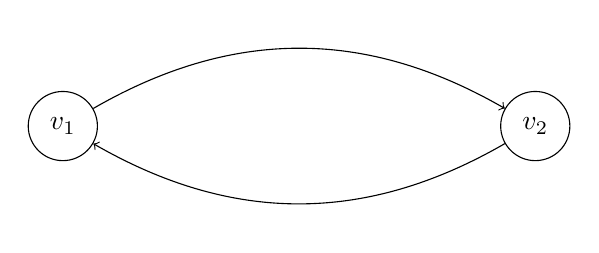
\begin{tikzpicture}[->, node distance = 3cm, auto]

          \node[state](v1)at(1,  0)  {$v_1$};
          \node[state](v2)at(7,  0)  {$v_2$};

          %%----------------------------------
          \path (v1)edge[bend left]node{}(v2)
          (v2)edge[bend left]node{}(v1);
          %%----------------------------------
        \end{tikzpicture}
      \end{center}

      Ahora, supongamos que hay un ciclo $C$ de al menos longitud $\delta^+ +1$
      con $\delta^+ > 1$, para $n(n > 1)$ vértices en $D$ y además $D$ no
      tiene lazos.
      
      Luego, para $|V_D| = n +1$ donde llamaremos $x$ al vértice
      extra.
      
      Analicemos dos casos extremos:

      \begin{itemize}
        \item[-] Si $x$ tiene una sóla incidencia, entonces $\delta^+ = 1$ y como
          $\mathcal{L}(C) > 1$, tenemos que existe un ciclo de al menos $\delta^+ +1$.
          En este caso, tenemos que es estrictamente mayor. 
          De lo anterior, terminamos. 

        \item[-] Si para cada vértice $u_i(1 < i \geq |V_D| -1)$ en $G$ hay
          una arista que ``salga" de $u_i$ e incida en $x$, tenemos que $\delta^+$
          no se modifica.
          
          Ahora notemos que, en partícular, hay al menos
          $u_i, u_{i +1}$ tales que existe una $u_i u_{i +1}$-trayectoria en $C$
          (notemos que $u_i$ y $u_{i +1}$ son vecinos). 
          Luego, como existe $e_1 = u_i x$ y $e_{2} = u_{i +1} x$, con $e_1$
          y $e_2$ en $E_D$, tenemos un nuevo ciclo que es de al menos
          $\mathcal{L}(C) +1$ de longitud. 
          Así, como $\mathcal{L}(C) \geq \delta^+ +1$, tenemos que el nuevo ciclo es
          de al menos longitud $\delta^+ +1$.
      \end{itemize}
      Del análisis anterior, concluimos que el enunciado se cumple.
    \end{proof}
  \end{enumerate}

  \section*{Puntos Extra}
  \begin{enumerate}
    %%%%%%%%%%%%%%%%%%%%%%%%%%%%%%%%%%% 01 EXTRA %%%%%%%%%%%%%%%%%%%%%%%%%%%%%%%%%%%
    \item Demuestre que el n\'umero de $v_i v_j$-caminos de longitud $k$ en $G$ es
      $(A^k)_{ij}$ donde $A$ es la matriz de adyacencia de $G$.
      \begin{proof} Inducción

        Paso base $(n=1)$ 
        
        Sea $V_i V_j$ adyacentes $\Longrightarrow A_{ij}=1$ y en caso de que no sean
        adyacentes $A_{ij}=0 \Longrightarrow$ lo que implica que el numero de caminos
        de longitud 1 entre $V_i V_j = A_{ij}= A^1_{ij} $
        
        Hipótesis de inducción $(n=k)$
        
        Supongamos que el número de  $V_i V_j -$caminos de longitud k en G es $(A^k)_{ij}$
        
        Paso inductivo $(n=k+1)$
        
        $Pd)$ El número de  $V_i V_j -$caminos de longitud $k+1$ en G es $(A^{(k+1)})_{ij}$
        
        Dem
        
        Sea $A^{(k+1)} = A^k * A \Longrightarrow$ por definición de multiplicacion de matrices sean
        "t" los elementos de la matriz $A^k$ y "a" lo elemntos de la matriz A
        $\Longrightarrow A^k * A = \sum_{r=1} t_{ir}a_{rj}$ paratoda $A_{ij}$ que pertenece a
        $A^{(k+1)} \Longrightarrow (A^{(k+1)})_(ij) = (A^k * A)_(ij) =  \sum_{r=1} t_{ir}a_{rj}$
        (Esta suma en especifico  es la multiplicación de un renglón de $A^k$ y una columna de A)
        
        $\Longrightarrow$ si $a_{rj}=0 \Longrightarrow V_r$ y $V_j$ no son adyacentes y por
        hipótesis de inducción $t_{ir}$ son el número de caminos que existen de longitud k
        de $V_i$ a $V_r$
        
        Caso 1) $a_{rj}=0$
        $\Longrightarrow$ ($t_{ir}*a_{rj}=0$) $\Longrightarrow$ existen 0 caminos de longitud  $n+1$
         
         Caso 2)  $a_{rj}=1$
         $\Longrightarrow$  ($t_{ir}*a_{rj}=t_{ir}$) $\Longrightarrow$ existe 1 camino de longitud
         $n+1$ que recorre de $V_i V_j$ 
        
         $\Longrightarrow  \sum_{r=1} t_{ir}a_{rj}$ independientemente de si $a_{rj}=0$ o $a_{rj}=1$
         nos dará el número de caminos de longitud $n+1$ que existen entre $V_i V_j$ 
        
        \end{proof}
    %%%%%%%%%%%%%%%%%%%%%%%%%%%%%%%%%%% 01 EXTRA %%%%%%%%%%%%%%%%%%%%%%%%%%%%%%%%%%%
    \item Sea $G$ una gr\'afica bipartita de grado m\'aximo $k$.   Demuestre que
      existe una gr\'afica bipartita $k$-regular, $H$, que contiene a $G$ como
      subgr\'afica inducida.
  \end{enumerate}
\end{document}
